\documentclass[letter, 12pt] {article}

\usepackage{tabularx}
\usepackage{graphicx}
\usepackage[french]{babel}
\usepackage[utf8]{inputenc}
\usepackage[french, vlined]{algorithm2e}
\usepackage{geometry}
\geometry{ hmargin=2.5cm, vmargin=2.3cm }

%%%%% Page titre %%%%


%%%% Résumé %%%%
%Pour la taille des interlignes
\renewcommand{\baselinestretch}{1.3}


\newlength{\larg}
\setlength{\larg}{15cm}

\title{
{\rule{\larg}{1mm}}\vspace{7mm}
\begin{tabular}{p{0cm} r}
& {\Huge {\bf Rapport d'activité}} \\
\end{tabular}\\
\vspace{2mm}
{\rule{\larg}{1mm}}
\vspace{2mm} \\~\\
\begin{tabular}{p{3cm} r}
& {\large \bf Projet transversal d'ingénierie objet - IG4} \\
& {\large \bf encadré par M. Stratulat} \\
& {\large 17 mars 2011}
\end{tabular}\\
\vspace{10cm}
}
\author{\begin{tabular}{p{5cm} l}
 Emmanuel Damiano & Quentin Dejean\\ 
 Raphael Pastou & Damien Vacher
\end{tabular}\\
\hline }
\date{}

\begin{document}

\maketitle
\thispagestyle{empty}

\tableofcontents

\newpage


\setcounter{page}{1}

	\section*{Introduction}
	
	\section{Le diagramme de classes}
	
	$Nous étudions ici la fonctionnalité permettant d'afficher (et ultérieurement d'imprimer) le PV d'une étape en cours. Nous partons du principe que les données de l'étape sur laquelle travaille la secrétaire sont chargées dans les classes. Ainsi, la fonctionnalité travaille directement sur l'étape sur laquelle se trouve la secrétaire (qui pourra changer entre les étapes dont elle s'occupe à tout moment).

	Nous disposons donc d'un diagramme de classe relativement simple. Une interface (pour l'instant seulement graphique) permet la communication entre le système et l'utilisateur, elle permettra de consulter le PV. Une façade est présente afin de réaliser la communication entre la partie interface et la partie Business Layer permettant de cacher la complexité à ce dernier. Dès lors, nous avons la classe principale de la fonctionnalité, la classe Process_PV, disposant d'une étape et des méthodes d'accès aux données. Ainsi, il peut récupérer l'intégralité des données d'une étape, essentielle à la création d'un PV.
		
		La partie persistance est sensiblement la même que celle pour l’ensemble du programme. Nous avons décidé d’omettre le pattern factory (pour le type de sauvegarde), non essentiel ici car on se contente de consulter les données des classes. Nous avons donc une classe structure contenant l’ensemble des données et méthodes généralisable entre UE, ECUE, Semestre et étape. Nous y retrouvons donc le code_structure, le libelle, une liste d’étudiant et une liste de note. En effet, cette dernière se retrouve dans toutes les classes, les notes des élèves pour l’ECUE, les moyennes des élèves pour l’UE, ainsi que pour le semestre et l’étape. Le reste des classes découlant de cette généralisation contiennent simplement leurs attributs qui leurs sont propres (un ECTS pour ECUE, des coefficients pour UE et semestre ainsi que des liste de points jury, ...)
		$$
		Une fois cette généralisation effectuée, les seuls points compliqués peuvent être les classes « Struct_note » et « Struct _mention ». C’est classe sont en réalité des structures de donnée permettant de contenir diverses informations. Dans notre cas, elles contiennent respectivement un couple ${étudiant, note_etudiant}$ et ${étudiant, mention_étudiant}$ ou « mention_étudiant » est un string qui contiendra ACQ, NACQ, ACDJ.
	
	\section{Les cas d'utilisation}
	
	\begin{figure}[htbp]
		\centering
			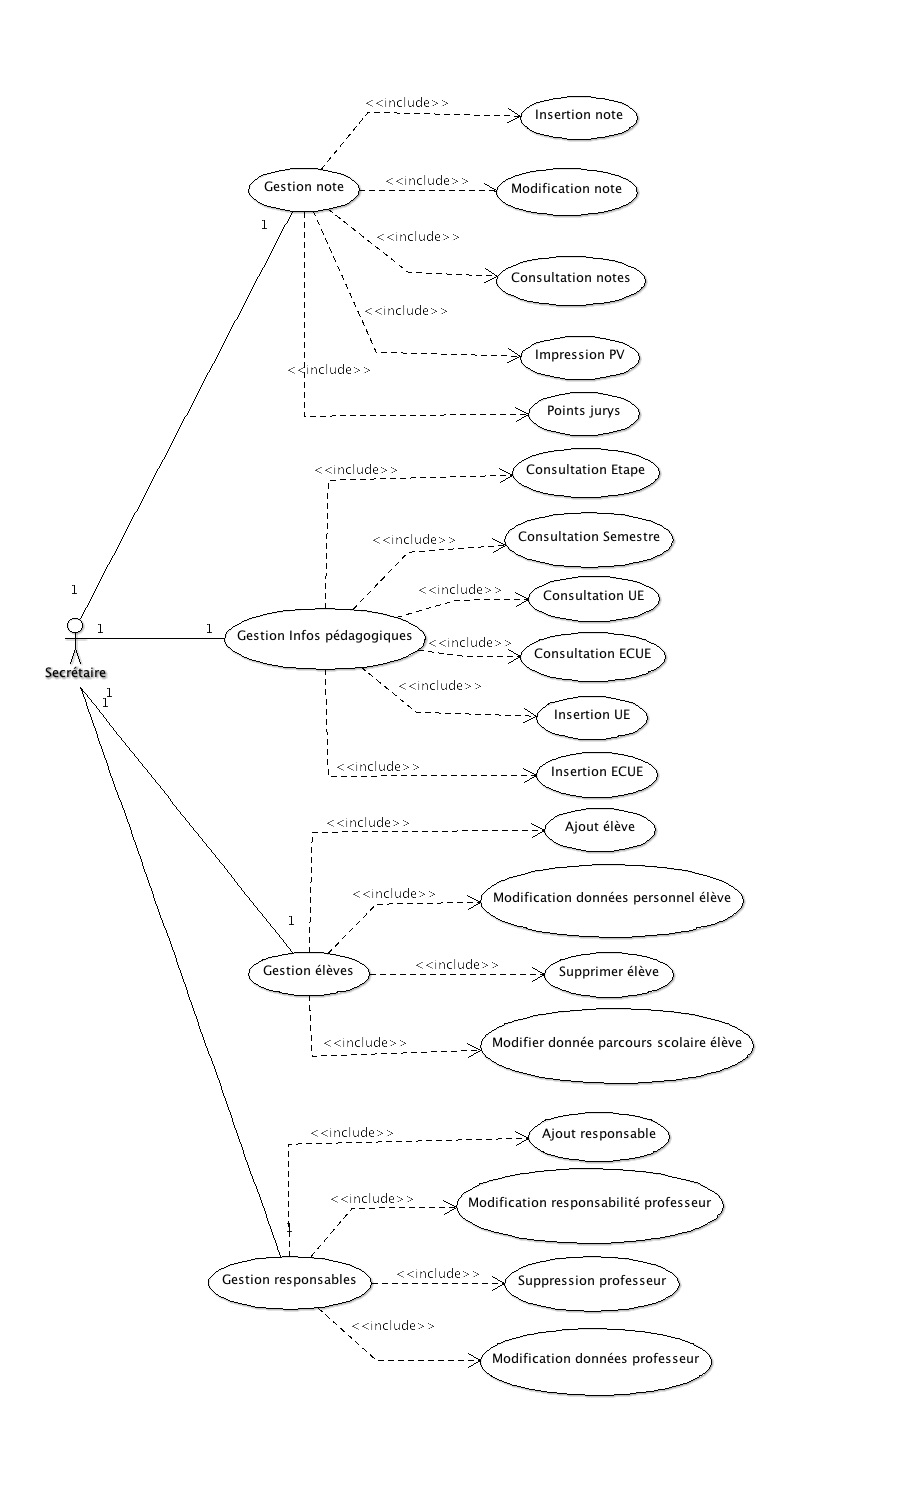
\includegraphics[scale = 0.5]{../Use_Case/Diagramme_Use_Case.png}
		\caption{Masque d'analyse des entreprises}
	\end{figure}
	
	\newpage
	
	Nous avons fait le choix de réaliser nos Use Cases sur deux niveaux. Au premier niveau, nous retrouvons les fonctionnalités de base de l'application. 
	
	Tout d'abord, la gestion des notes, qui réunit l'insertion, la modification ou la consultation des notes des étudiants.
	Ici, nous ne prenons pas en compte la gestion des notes de rattrapage, car si un étudiant doit rattraper une matière, la secrétaire ne fera que modifier la note principale par la note qui lui sera communiquée par le responsable de l'ECUE. C'est aussi au sein de la gestion des notes que la secrétaire pourra imprimer le PV.
	
	Ensuite viennent les informations qui concernant la gestion des informations pédagogiques. Il est donc possible de consulter l'ensemble des structures des enseignements, mais aussi d'insérer une UE ou une ECUE si nécessaire.
	
	La troisième fonctionnalité correspond à la gestion des élèves. Ainsi, il sera possible de modifier uou supprimer un élève.
	
	Pour terminer, la dernière fonctionnalité concerne la gestion des responsables, avec toutes les caractéristiques que cela concerne.
	
	\section{Les diagrammes de collaboration}
	
	\section{Les diagrammes de séquence}
	
	\section{Le diagramme d'activité}
	
	\section{Conclusion du rapport préliminaire}
	
		
		
\end{document}